
\documentclass[conference]{IEEEtran}

\usepackage[pdftex]{graphicx}
\usepackage{amsmath}

\graphicspath{IEEEtran/images/}
\DeclareGraphicsExtensions{.pdf,.jpeg,.png,.PNG}

\usepackage{multirow}
% *** CITATION PACKAGES ***
%
\usepackage{cite}

\renewcommand{\tablename}{Tabla}
\renewcommand{\abstractname}{Resumen}
\renewcommand{\IEEEkeywordsname}{Palabras clave}
\renewcommand{\refname}{Referencias}
\usepackage{pythontex}
\usepackage{caption}
\usepackage{subcaption}
\usepackage[flushleft]{threeparttable}
\hyphenation{op-tical net-works semi-conduc-tor}

\begin{document}

\title{Aprendizaje automático y la atención al cliente}
\author{\IEEEauthorblockN{Eliécer Mora-Alaniz}
\IEEEauthorblockA{Tecnológico de Costa Rica\\
Escuela de Ingeniería Electrónica\\
MP-6122 Reconocimiento de Patrones\\
email: eliecer@estudiantec.cr}}

\maketitle

\begin{abstract}
The machine learning field can be applied to many areas. The customer service area has found a way to reduce costs and improve the quality of its services through the machine learning. In this paper the main applications of machine learning in the customer service area are presentend to provide a general idea of the application of in this field.
\end{abstract}

\begin{IEEEkeywords}
Customer Support, Machine Learning
\end{IEEEkeywords}

\section{Introducción}

En este artículo se presentan algunas de las aplicaciones principales del aprendizaje automático en el área del servicio al cliente.

La metodología empleada consiste en indagar las aplicaciones que se tienen actualmente en la industria del servicio al cliente, así como los retos que se plantea la industria para mejorar la calidad y productividad del servicio brindado.

En los últimos años se ha presentado el aprendizaje automático como tendencia en muchos ámbitos. El servicio al cliente, al ser un área en la que se tienen muchos procesos automáticos, presenta un nicho importante para esta tecnología \cite{11cases, hbr, airole}.

Se detectaron al menos los siguientes casos de uso:
\begin{itemize}
\item Identificación de problemas del cliente por escucha social y soluciones de etiquetado.
\item Autenticación de usuarios por medio de biométrica.
\item Asignación de agentes.
\item Automatización de actividad de los agentes.
\item Chatbots.
\item Detección de fraude.
\item Analítica.
\end{itemize}

Existen algunas áreas emergentes como lo es la traducción en tiempo real.

\section{Identificación de problemas de clientes}

La identificación de un problema en el momento en que este aparece es el primer paso para resolver la problemática. El \textit{social listening} o monitoreo de las redes  sociales \cite{socialmonitorcompare} ayudan a aprovechar el procesamiento del lenguaje natural para así identificar clientes que deben ser contactados y brindarles una respuesta automática, o si fuese el caso, asignar agentes específicos permite incrementar la satisfacción del cliente. \cite{11cases}.

El monitoreo de las redes sociales puede incluso incrementar el promedio de consumo por cliente. Se sabe que los clientes que se comprometen con las compañías por medio de las redes sociales invierten entre un 20\% a un 40\% más de dinero en estas compañías respecto a otros clientes \cite{socialmonitor}. Por otro lado, esta herramienta permite reducir los costos por contacto con el cliente hasta en un 83\% \cite{mckinsey, whysocialmonitor}.

Además, el monitoreo de las redes sociales permite extraer búsquedas específicas de los clientes por medio de sus comentarios en las redes sociales para así clasificar la consulta y determinar la respuesta que mejor se ajusta a un modelo de aprendizaje, ya sea supervisado o no supervisado \cite{8703237}. Cabe rescatar que según distintos estudios realizados, los métodos supervisados han mostrado un mejor desempeño en la clasificación de consultas \cite{8703237}.

\section{Autenticación de usuarios con biometría}

Debido a la alta incidencia de casos en los que los usuarios sufren estafas por suplantación de identidad (principalmente por ingeniería social), han surgido nuevos métodos de autenticación en los que se emplean características o atributos físicos de la persona para validar su identidad en sitios o aplicaciones. Los métodos incluyen desde lectores de huellas digitales, reconocimiento de retina, iris o cara, detección de voz hasta detectores de vida.

Estos últimos responden al contra ataque de los métodos empleados por los suplantadores de identidad, ya que una manera de engañar a los sistemas de autenticación consiste en colocar imágenes en dos dimensiones frente al detector de cara, retina o iris. \cite{biometric}
En el caso del reconocimiento de voz, las soluciones consisten en traducir palabras en una huella de voz que es única para una persona. De esta manera se puede asegurar la autenticación de un cliente.

\section{Asignación de agentes}

El modelado del comportamiento de los clientes permite predecir mediante modelos de aprendizaje automático el comportamiento que el cliente podría presentar y de esta manera asignar al agente que sea más acertado según sus características para que atienda a esta persona. Esto permite que al atención para el cliente sea mejor, ya que es atendido por un agente con la experiencia y el estilo que concuerda con las necesidades del cliente.

Esta aplicación presenta varios retos que han sido atendidos en \cite{user_modeling}, siendo algunos de ellos la necesidad de conjuntos de datos grandes y de datos etiquetados, el corrimiento de concepto y la complejidad computacional.

Aún más, los sistemas de clasificación de llamadas emplean el procesamiento del lenguaje natural para determinar lo que un cliente quiere decir y de esta manera le permite a los agentes enfocarse en actividades de mayor valor agregado y a la vez permite mejorar la asignación de agentes a los usuarios \cite{11cases}.

Este problema ha sido atacado por medio de métodos de aprendizaje no supervisado \cite{9254369} y semi-supervisado para así segmentar a los clientes según distintos atributos.

Los sistemas de enrutamiento de llamadas son otro ejemplo de aplicar el aprendizaje automático al área de servicio al cliente. Estos permiten asignar las llamadas a los agentes disponibles que se encuentran mejor capacitados. Estos sistemas emplean los datos de todas las interacciones con los usuarios para así optimizar la satisfacción del cliente \cite{11cases}.

\section{Automatización de actividad de los agentes}

Se han aplicado distintos métodos para clasificar las consultas realizadas por lo clientes de manera que se puede determinar la categoría de una consulta según distintas palabras en la consulta. Varios estudios han obtenido resultados con una precisión del 65\% en la discriminación de consultas \cite{8554881}, mostrando a la máquina de vectores de soporte como un método que muestra los mejores resultados en comparación con otros métodos tradicionales de clasificación.

Al aplicar el aprendizaje automático en las actividades  permite ahorrar el tiempo de los agentes mientras que a la vez se incrementa la satisfacción del cliente. El procesamiento de lenguaje natural y el aprendizaje automático se emplea para estimar y gestionar los intentos de los clientes. Esto a la vez permite que el servicio al cliente brinde la asistencia que el usuario necesita y en la manera en que ellos quieren. Esto permite mejorar las métricas de satisfacción de los clientes y del negocio \cite{microsoft, ubercota, 8703237}.

\begin{figure}
\centering
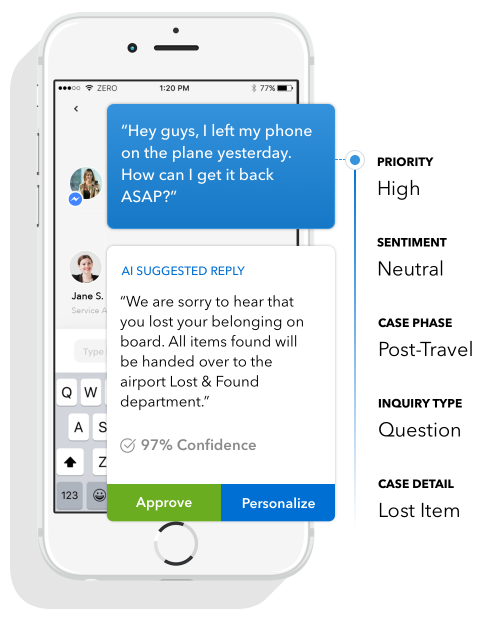
\includegraphics[width=8cm]{IEEEtran/images/response_suggestion.png}
\caption{Sugerencia automatizada de respuesta al cliente. Tomado de \cite{digitalgenius}.}
\label{fig:response_suggestion}
\end{figure}

Aún más, existen soluciones que permiten estimar las emociones de los clientes al analizar señales visuales, de texto y auditivas de los clientes. Esto permite que los agentes sean más conscientes de las emociones de los clientes y así poner atención a los clientes que así lo requieran. Además, existen aplicaciones en las que un robot monitorea las conversaciones\cite{digitalgenius, ubercota} para así brindar sugerencias en tiempo real sobre las respuestas que se le pueden brindar al cliente y así mejorar la satisfacción del usuario y estandarizar la experiencia de éste, la figura \ref{fig:response_suggestion} presenta un ejemplo de esta tecnología aplicada.

\section{Chatbots}

Según varios estudios \cite{chatbotsresearch}, alrededor del 20\% de los negocios que emplean chatbots, los emplean para dar soporte al departamento de servicio al cliente y es la tercera aplicación más empleada después del departamento de tecnologías de información.

\begin{figure}
\centering
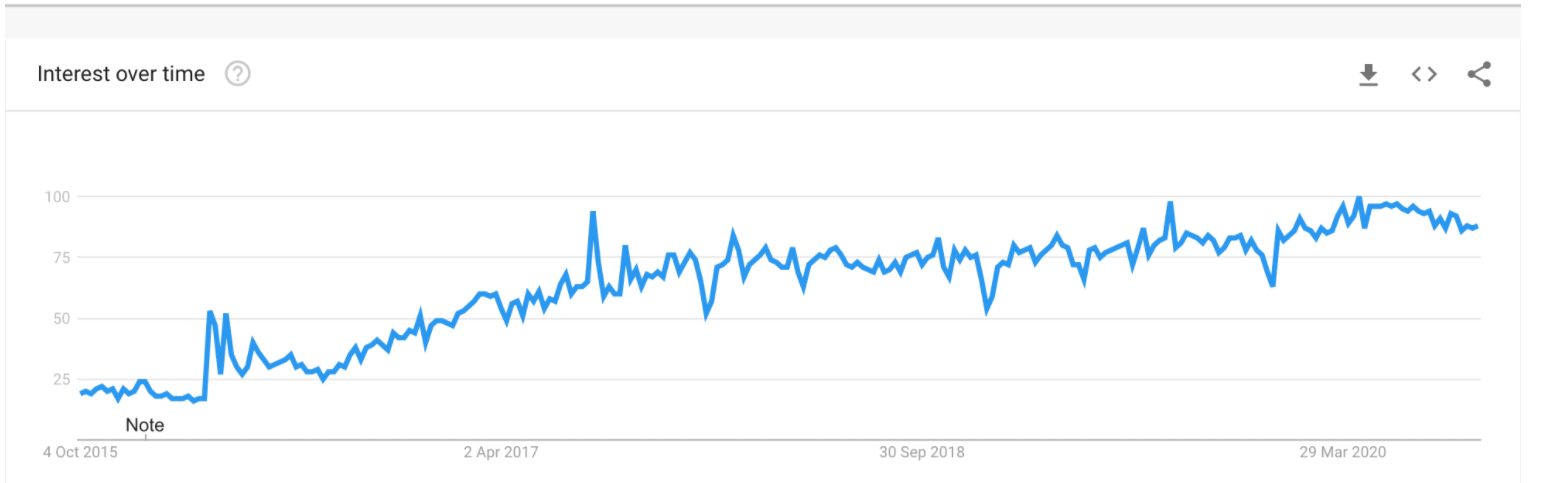
\includegraphics[width=8.5cm]{IEEEtran/images/chatbot_interest.png}
\caption{Interés de las empresas en los chatbots. Tomado de \cite{chatbotsresearch}.}
\label{fig:chatbot_interest}
\end{figure}

Esto no es completamente una sorpresa, ya que el 75\% de los clientes considera que toma mucho tiempo el hacer contacto con un representante de servicio al cliente humano. Por otro lado, la figura \ref{fig:chatbot_interest} muestra que alrededor del 100\% de las empresas están interesadas en los chatbots. Esto no es de sorprenderse ya que esta tecnología basada en el procesamiento del lenguaje natural \cite{ubercota, 9325440} permite reducir costos y mejorar la calidad del servicio al cliente. Producir una herramienta de este tipo requiere de una inversión considerable \cite{9322667} y se debe considerar el ciclo de pruebas dentro de la etapa de desarrollo para asegurar una buena tasa de retorno de la inversión \cite{chatbottesting, chatbottestingframework}.

En la actualidad, se han probado acercamientos por medio de redes neuronales convolucionales para detectar imágenes y así plantear un chatbot capaz de responder a consultas de artículos por medio de imágenes \cite{9335874}.

\section{Detección de fraude}

Esta aplicación no está relacionada directamente con la interacción con el cliente. Sin embargo, dada la cantidad de nuevas formas de estafa y fraude bancario, esta capacidad se vuelve necesaria para los clientes. El detectar una transacción fraudulenta presenta un servicio necesario para los clientes bancarios en la actualidad \cite{9182954, 9342475}. Esta tarea consiste en emplear los métodos de aprendizaje automático para clasificación, de tal modo que una transacción entre todas las transacciones de un cliente, sea discriminada como válida o fraude.

Se tiene referencia de métodos que van desde aplicaciones basadas en web \cite{9182954}, en los que se concluye que es necesario emplear redes neuronales convolucionales para mejorar los resultados, pasando por las redes de K vecinos cercanos \cite{7972424} y la detección de valores atípicos, hasta aplicar métodos de ingeniería de atributos y marcos de trabajo de la mejora del gradiente \cite{9342475} (como catBoost) para obtener resultados prometedores de alrededor del 98.3\% de exactitud en la predicción.

\section{Analítica}

Uno de los grandes retos dentro de la industria del servicio al cliente es el análisis de los datos. Y claramente, la manera de proveer los datos necesarios para los modelos de aprendizaje automático es recogerlos y procesarlos, para obtener información respecto a ellos. Incluso, el uso del aprendizaje automático y la interacción con los usuarios genera nuevos datos que deben analizarse para determinar el comportamiento y la aceptación de los métodos aplicados. Algunos ejemplos en los que se puede obtener información para analizar es en los chatbots, las llamadas telefónicas, las encuestas y revisiones que realizar los clientes.

El aprendizaje automático, en la rama del procesamiento de lenguaje natural, se puede aplicar para procesar todos estos datos y obtener información útil para las empresas.

\section{Nuevos retos}

Son innumerables los campos en los que se puede innovar en cuanto a la atención al cliente. Sin embargo, hay ideas sobresalientes que deben seguir investigándose pues el potencial que representan es mucho. Un ejemplo de esto es el uso del aprendizaje automático para procesar el lenguaje de señas por medio de vídeo en tiempo real y producir texto a partir de este vídeo. A la vez, tomar texto y producir a partir de este algún tipo de traducción a lenguaje a señas. Esto permite crear una interfaz entre una persona no oyente (que emplea lenguaje a señas) y una persona que no conoce el lenguaje a señas. Y, aunque la aplicación ya fue presentada \cite{lingvo}, se requiere de datos de prueba para mejorar la precisión del sistema, que a pesar de ser reciente, muestra precisiones entre el 70\% y 80\%.

\section{Conclusiones y recomendaciones}

El empleo de los métodos de aprendizaje automático en la escucha o el monitoreo de redes sociales permite clasificar las necesidades o problemas de los clientes de una manera oportuna para así brindar una solución temprana que resuelva la necesidad del usuario.

Los métodos de autenticación de usuarios por medio de atributos físicos o datos biométricos que emplean aprendizaje automático, permiten reducir la suplantación de identidad y a la vez facilitan la autenticación de los usuarios al no requerir recordar contraseñas para autenticarse en los distintos servicios brindados a los usuarios.

El uso del procesamiento del lenguaje natural permite predecir el comportamiento de un cliente para así asignar a un agente que sea adecuado para atender al usuario. Además, los sistemas de clasificación de llamadas permiten conocer la verdadera intención y sentimiento de un cliente por medio del análisis de la voz en tiempo real.

Al aplicar algoritmos de clasificación según el análisis aplicado a las consultas de los clientes, se automatiza la categorización de una pregunta sin la interacción de un agente de servicio al cliente. Esto permite reducir los costos y mejorar la velocidad de atención al usuario.

Además, al aplicar métodos de procesamiento en tiempo real de llamadas y/o conversaciones, se pueden brindar respuestas que automatizan el trabajo de un agente de servicio al cliente brindándole respuestas que corresponden a la consulta del usuario.

Los robots de conversaciones permiten reducir los costos en la atención al usuario y mejoran considerablemente el tiempo de respuesta de los usuarios. Sin embargo, es necesario que se invierta en el entrenamiento adecuado de estos robots para obtener los resultados esperados.

Los métodos de aprendizaje automático permiten la clasificación de transacciones bancarias para así detectar operaciones que pueden ser fraude en función de las características de la operación.

El procesamiento de lenguaje natural es ampliamente empleado en la industria de servicio al cliente debido a la interacción intrínseca con el ser humano de esta actividad.
Por otro lado, las oportunidades que tiene el aprendizaje automático para solventar problemáticas de la industria del servicio al cliente son muy prometedoras y abren una ventana a nuevas oportunidades de negocio.

\bibliographystyle{IEEEtran}
\bibliography{biblio}

\end{document}